\chapter{Underactuated Controller Design}
\label{chap:underactuated_controller}

\section{Introduction}
The underactuated system described in \autoref{chap:modelling} is a highly non-linear system thus traditional LTI control methods are not directly applicable. As discussed as part of the literature review in chapter \ref{chap:literature_review}, the backstepping controller is a suitable control method for underactuated systems. In this chapter, the underactuated backstepping controllers designed by Nadafi and Kabganian \cite{nadafiRobustBacksteppingAttitude2021} is analysed and its properties are discussed. A key defining feature of this controller is that it can achieve attitude tracking control i.e.: tracking a desired attitude profile under certain constraints, where most works are limited to regulation. It will be shown that this controller is robust to external disturbances, varying moment of inertia, reaction wheel torque disturbances and is performant in contrast to a control method such as model predictive control. This latter benefit is highly valuable on limited compute resources such as a satellite. This chapter will also discuss the controllability of the underactuated system and the limitations of the backstepping controller. A possible future modification to this controller is discussed using a technique developed by Haochang Tian in \cite{tianUnderactuatedTethered}. This controlle uses a similar backstepping methodology but contains a modification to the kinematic virtual control input to excite the actuated axes during a slew manoeuvre. Finally simulation results are presented which illustrate key constraints of the design.

\begin{comment}
 @TODO: Do I include input shaping in this chapter?
 An input shaping techinque is presented to achieve smooth point to point manoeuvres. This is then combined with a box manoeuvre to .
\end{comment}
\section{Controllability}
As mentioned in section \ref{underactuated_lit_review}, a controllability analysis of an underactuated satellite is presented in \cite{aeyelsStabilizationNonLinear} by Aeyels and Dirk. They show that a satellite with 2 reaction wheels is globally asymptotically stable by either a discontinuous or a smooth, time varying control law feedback control law. It is also shown that it is not controllable via a smooth time invariant control law. The authors prove that their proposed control law can achieve global asymptotic stability for the system via the central manifold theorem. They also show that a key requirement is that the angular momementum of the satellite must be zero $H = 0$ in order to achieve stability.

Nadafi and Kabganian \cite{nadafiRobustBacksteppingAttitude2021}, \cite{tianUnderactuatedTethered} and \cite{zarouratiUnderactuatedFaultTolerantControl} build on this work and present time-varying backstepping controllers.

\section{Backstepping}
\label{subsec:backstepping_procedure}
In order to understand the backstepping controller designed by Nadafi and Kabganian \cite{nadafiRobustBacksteppingAttitude2021}, it is necessary to understand the backstepping procedure. Backstepping is a non-linear design technique for stabilizing the origin of a system in strict-feedback form. It entails designing a series of virtual control inputs each of which stabilizes a subsystem and ultimately the overall system. The method is recursive in that the controller for the $i^{th}$ subsystem depends on the controller for the $(i-1)^{th}$ subsystem. The satellite kinematic and dynamic equations represent a 2nd order cascade system. A Lyapunov function is selected for each subsystem and the control law is designed to force the time derivative to this surface.

The satellite attitude kinematics and dynamics can be viewed as two subsystems connected in cascade: the dynamics subsystem is driven directly by the control input $\vec{u}$, while the kinematics subsystem is driven only indirectly, through the angular velocity produced by the dynamics subsystem. This mirrors the general backstepping structure of equation \eqref{eq:1}, with the dynamics playing the role of the inner subsystem $i$ and the kinematics playing the role of the outer subsystem $i-1$ whose virtual control input is designed first. This simplified cascade structure is illustrated in Figure~\ref{fig:cascade_simplified}; the full expressions for $f$ and $g$ are given later in this chapter once the underactuated case has been introduced (equations \eqref{eq:cascade_dyn} and \eqref{eq:cascade_kin}).

\begin{figure}[h]
    \centering
    \begin{tikzpicture}[
        block/.style={draw, minimum width=3.6cm, minimum height=1.3cm, align=center},
        node distance=2.4cm,
        >=Latex
    ]
        \node[block] (dyn) {$\dot{\vec{\omega}} = g(\vec{q},\vec{\omega}) + \vec{u}$};
        \node[block, right=of dyn] (kin) {$\dot{\vec{q}} = f(\vec{q},\vec{\omega})$};

        \draw[->] ($(dyn.west)+(-1.4,0)$) -- node[above]{$\vec{u}$} (dyn.west);
        \draw[->] (dyn.east) -- node[above]{$\vec{\omega}$} (kin.west);
        \draw[->] (kin.east) -- ++(1.4,0) node[right]{$\vec{q}$};

        \node[draw, dashed, inner sep=0.35cm, fit=(dyn), label={above:Subsystem $i$}] {};
        \node[draw, dashed, inner sep=0.35cm, fit=(kin), label={above:Subsystem $i-1$}] {};
    \end{tikzpicture}
    \caption{Simplified cascade block diagram of the satellite attitude dynamics (subsystem $i$) and kinematics (subsystem $i-1$).}
    \label{fig:cascade_simplified}
\end{figure}

\subsection{Lyapunov Functions}
To prove the stability of a non-linear system around an equilibrium point, a Lyapunov function is used. An equilibrium point is stable if all solutions starting close to the equilibrium point remain close to it for all time. An equilibrium point is asymptotically stable if it is stable and all solutions starting close to the equilibrium point converge to it as time goes to infinity. A Lyapunov function is a scalar function that is used to prove the stability of an equilibrium point of a dynamical system. It is a mathematical tool that provides a way to analyze the behavior of a system without explicitly solving its equations of motion. The basic idea behind Lyapunov functions is to find a function that decreases over time along the trajectories of the system, indicating that the system is moving towards a stable equilibrium point. Formally, let x = 0 be an equilibrium point of the system $\dot{x} = f(x)$ where $f : D \rightarrow \mathbb{R}^n$ is a locally Lipschitz map from a domain $D \subset R$ into $\mathbb{R}^n$ containing $x=0$.

which has an equilibrium point at $x=0$. The equilibrium point is stable if for each $\epsilon > 0$, there exists a $\delta > 0$ such that if $\|x(0)\| < \delta$, then $\|x(t)\| < \epsilon$ for all $t \geq 0$.

\input{chapter_4/lypunov_stability}
% @TODO: Fix this


 A Lyapunov function is a scalar function $V : D \rightarrow \mathbb{R}$ that is continuously differentiable and satisfies the following conditions:
\begin{equation}
    V(0) = 0, \quad V(x) > 0 \quad \forall \ x \in D, x \neq 0
\end{equation}
\begin{equation}
    \dot{V}(x) \leq 0 \quad \forall \ x \in D
\end{equation}
then x is stable. If
\begin{equation}
    \dot{V}(x) < 0 \quad \forall \ x \in D, x \neq 0
\end{equation}
then x is asymptotically stable. If D = $\mathbb{R}^n$ and V is radially unbounded then x is globally asymptotically stable \cite{khalilNonlinearSystems2002}.

 A Lyapunov function $V(\vec{x})$ is positive definite if $V(0)=0$ and $V(\vec{x})>0$ for all $\vec{x}\neq0$. It is radially unbounded if $V(\vec{x})\rightarrow\infty$ as $\vec{x}\rightarrow\infty$. A Lyapunov function is used to prove the stability of a system by showing that the time derivative of the Lyapunov function is negative definite ie: $V(\vec{x}) \leq -W(\vec{x})$ where $W(\vec{x})$ is a positive definite function. That is $\dot{V}(\vec{x})<0$ for all $\vec{x}\neq0$. If this is true then the system is stable. 

A common Lyapunov function chosen for electro-mechanical systems is the total energy of a system (pendulums, robot manipulators, converters, ship dynamics), since total energy V = kinetic + potential is already a natural positive-definite candidate. However this is not a requirement and other Lyapunov functions can be used along as it satisfies the conditions of being positive definite and differentiable \cite{khalilNonlinearSystems2002}.
\subsection{Backstepping Procedure}
Using the Lyapunov stability theory, the backstepping procedure as outlined in \cite{khalilNonlinearSystems2002} can be described as follows. Take the following 2nd order equation:

\begin{equation}
    \dot{\eta} = f(\eta) + g(\eta)\xi \label{eq:1}
\end{equation}
\begin{equation}
    \dot{\xi} = u
\end{equation}

where $f(0)=0$ and g is non-zero over the region of interest.
The goal is to design a control law $u$ such that the origin $\eta=0$ is asymptotically stable i.e.: $(\eta, z)$ returns to $(0,0)$ after starting from some arbitrary initial condition.

Assuming that equation \eqref{eq:1} can be stabilized by a smooth feedback state feedback law $\xi=\phi(\eta)$ with $\phi(0)=0$ such that 

$$
    \dot{\eta} = f(\eta) + g(\eta)\phi(\eta)
$$

and assuming that there is a Lyapunov function $V(\eta)$ which stabilizes the subsystem then it should satisfy

\begin{equation}
\dot{\eta} = \frac{\partial V}{\partial \eta}[f(\eta) + g(\eta)\phi(\eta)] \leq -W(\eta), \quad \forall \ \eta \in D
\end{equation}

where $W(\eta)$ is a positive definite function. As we will see later $V$ can be chosen to suit application specific needs of the system.

We can then obtain the equivalent expression by adding and subtracting $g(\eta)\phi(\eta)$ on the righthand side of equation \eqref{eq:1}:
\begin{equation}
    \dot{\eta} = [f(\eta) + g(\eta)\phi(\eta)] + g(\eta)[\xi - \phi(\eta)] 
\end{equation}

The above is repsented in figure \ref{fig:backstepping} b). The change of variables 
$$ z = \xi - \phi(\eta) $$
results in the system 

$$ \dot{\eta} = [f(\eta) + g(\eta)\phi(\eta)] + g(\eta)z  $$
$$ \dot{z} = u - \dot{\phi} $$

which is shown in Figure \ref{fig:backstepping} c). Going from step b) to c) is called backstepping because you are backstepping the control input $-\phi(\eta)$ through the integrator. Finding the derivative $\dot{\phi}$ 

$$ \dot{\phi} = \frac{\partial \phi}{\partial \eta} [f(\eta) + g(\eta)] $$

and taking $v = u - \dot{\phi}$ we obtain the cascade connection

$$ \dot{\eta} = [f(\eta) + g(\eta)\phi(\eta)] + g(\eta)z  $$
$$ \dot{z} = v $$

This modified system is similar to the starting system however now the inner subsystem has an asymptotically stable origin when the input is zero. We can now choose a candidate Lyapunov function for the overall system:

$$ V_c (\eta,\xi) = V(\eta) + \frac{1}{2}z^2 $$

from which we obtain
\begin{align}
    \dot{V_c} &= \frac{\partial V}{\partial \eta}[f(\eta) + g(\eta)\phi(\eta)] + \frac{\partial V}{\partial \eta}g(\eta)z + zv \\
    &\leq -W(\eta) + \frac{\partial V}{\partial \eta}g(\eta)z + zv
\end{align}

Choosing $v$ such that it cancels out the 2nd last term from the above

$$ v = -\frac{\partial V}{\partial \eta}g(\eta) - kz, \; k > 0 $$

gives us

$$ \dot{V_c} = -W(\eta) - kz^2 $$

where k influences the rate of convergence.
This shows that the origin $(n=0, z=0)$ is asymptotically stable. Since $\phi(0) = 0$ we know that the origin $(n=0, \xi=0)$ is also asymptotically stable. Substituting for $v$, $z$ and $\phi$ we obtain the control law for the system:

\begin{equation}
    u =  \frac{\partial \phi}{\partial \eta} [f(\eta) + g(\eta)\xi] - \frac{\partial V}{\partial \eta}g(\eta)z - k[\xi - \phi(\eta)]
\end{equation}

If all assumptions hold globally and $V(\eta)$ is radially unbounded then that origin is globally asymptotically stable.
This idea can be extended to higher order systems.

\par
This process can be visualized in figure \ref{fig:backstepping}.

\begin{figure}
    \centering
    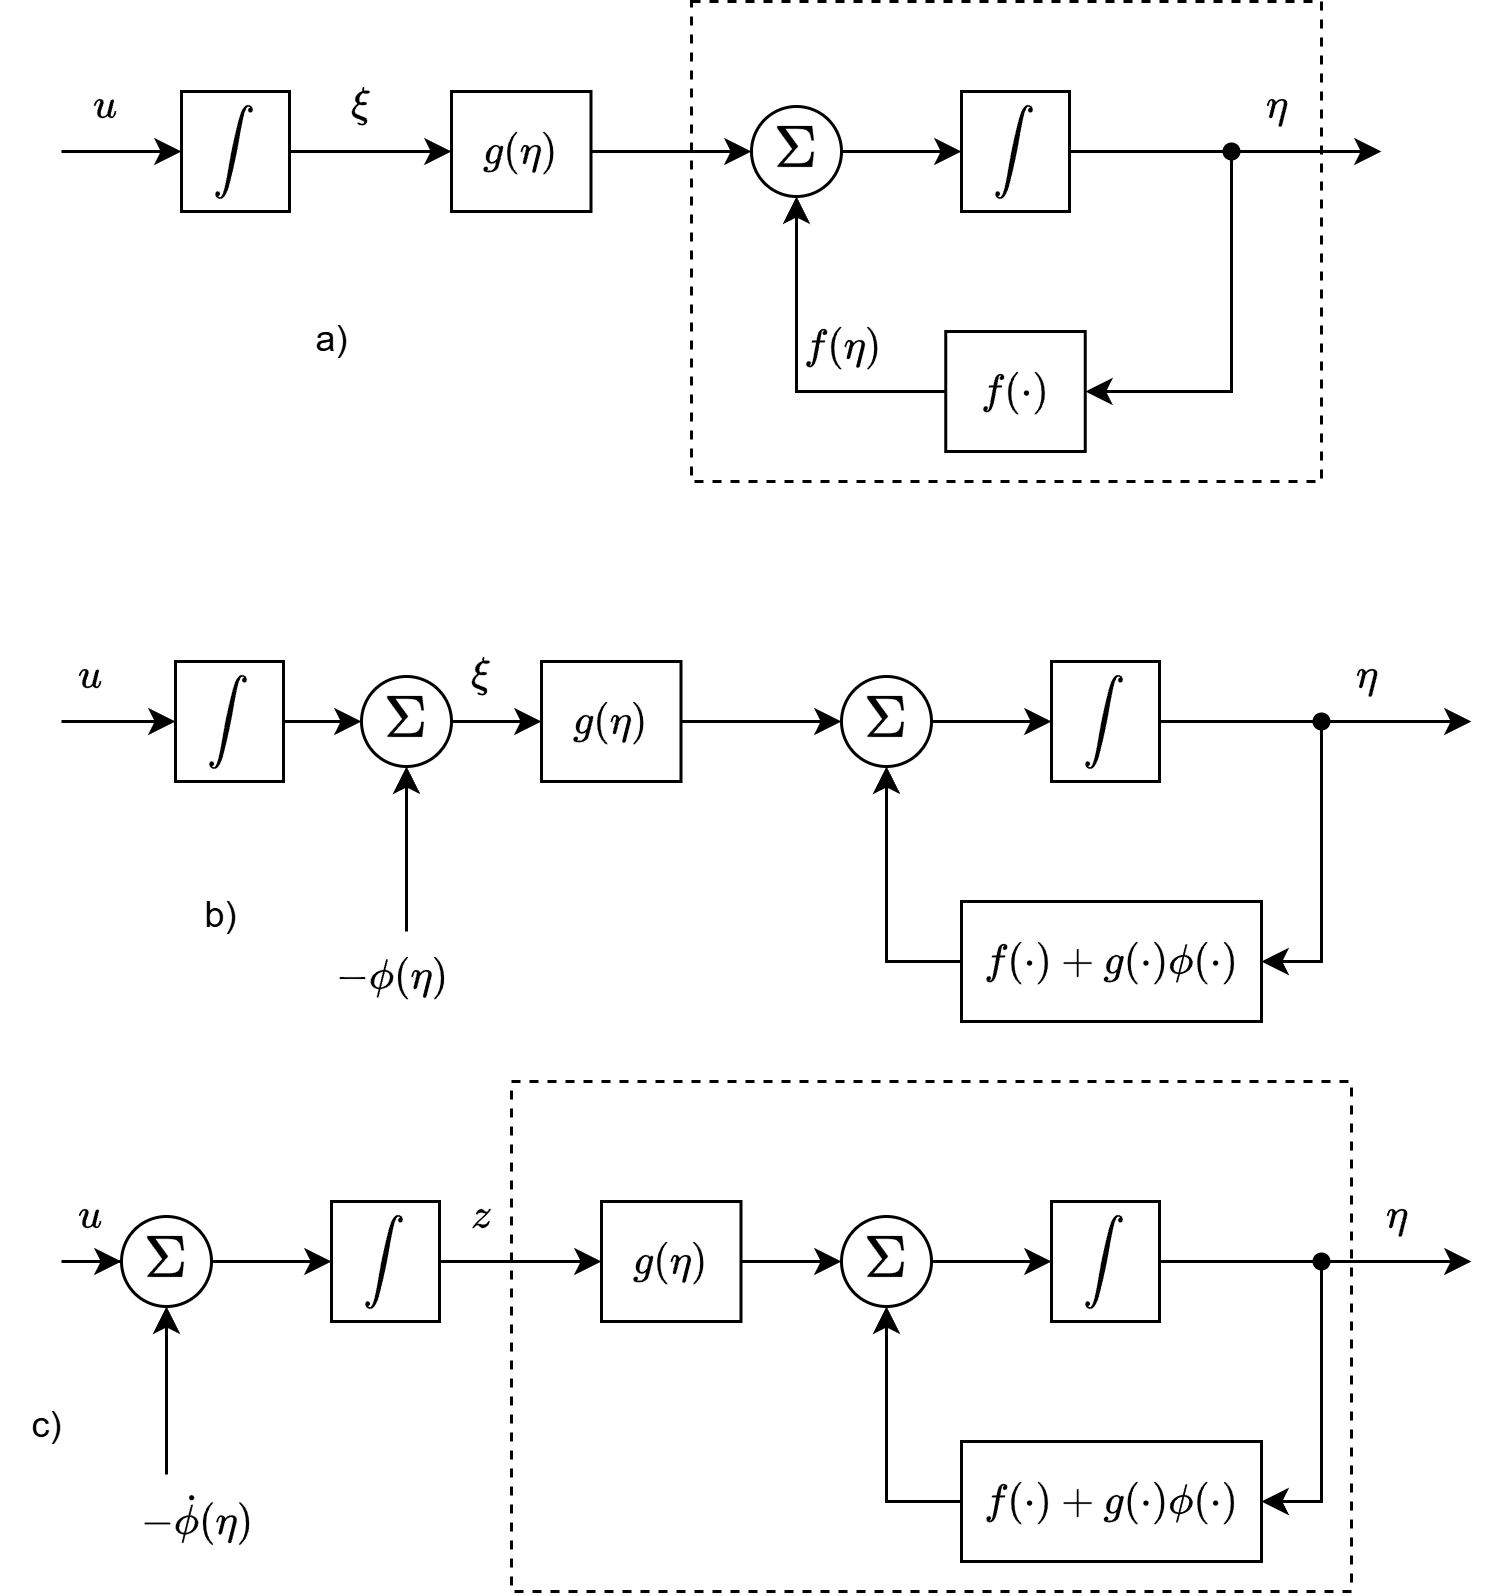
\includegraphics[width=1.0\textwidth]{chapter_4/Backstepping_diagram.drawio.png}
    \caption{Backstepping visualization block diagram series. a) Original system b) Introduce virtual control input c) Backstepping control input through integrator}
    \label{fig:backstepping}
\end{figure}
\newpage
\section{Nadafi and Kabganian Controller}

Nadafi and Kabganian \cite{nadafiRobustBacksteppingAttitude2021} present a robust backstepping attitude tracking controller for an underactuated spacecraft equipped with two reaction wheels, addressing the coupled kinematic--dynamic (cascade) model in the presence of actuator saturation and time-varying perturbations. The key contribution is a novel hypersurface that stabilises the unactuated attitude degrees of freedom via virtual inputs, enabling full asymptotic convergence of both angular velocity error and quaternion error using only two torques. They require no limitations on the reference quaternion.

\subsection*{Cascade Model}

Under the assumptions (z-axis is the unactuated axis; total angular momentum is zero so $\omega_z = 0$), the full spacecraft dynamics reduce to a two-part cascade system in the actuated angular velocity error $\boldsymbol{\omega}^r_e = [\omega_{ex},\, \omega_{ey}]^T \in \mathbb{R}^2$ and the quaternion error $\vec{q}_e \in \mathbb{R}^4$:
\begin{align}
    \dot{\boldsymbol{\omega}}^r_e &= \vec{u} + \vec{F} + \vec{d} \label{eq:cascade_dyn} \\
    \dot{\vec{q}}_e &= A(\vec{q}_e)\,\boldsymbol{\omega}^r_e, \quad
    A(\vec{q}_e) = \frac{1}{2}\begin{bmatrix}
        q_{e0} & -q_{e3} \\
        q_{e3} &  q_{e0} \\
       -q_{e2} &  q_{e1}
    \end{bmatrix} \label{eq:cascade_kin}
\end{align}
where $\vec{u} = \{J^r_0\}^{-1}\dot{\vec{h}}^r_w \in \mathbb{R}^2$ is the control input (reaction wheel torque), $\vec{F} = - \vec{C}^r \vec{\dot{\omega}}_d^r + \{ c_{31} \omega_{dx} + c_{32} \omega_{dy} \} [\omega_{ey} \ -\omega_{ex}]^T$ captures the known gyroscopic and reference-trajectory terms, and $\vec{d}$ is the total bounded perturbation, which includes external disturbances, time-varying inertia uncertainty $\Delta J$, and internal reaction wheel disturbances.

\subsection*{Disturbance Observer}

To estimate $\vec{d}$, a finite-time nonlinear disturbance observer (FNDO) is employed:
\begin{align}
    \dot{\boldsymbol{\chi}}_0 &= \boldsymbol{\nu}_0 + \vec{u} + \vec{F}, \quad
    \boldsymbol{\nu}_0 = -\kappa_0\,\mathrm{diag}\!\left(L^{1/2}|\boldsymbol{\chi}_0 - \boldsymbol{\omega}^r_e|^{1/2}\right)\mathrm{sign}(\boldsymbol{\chi}_0 - \boldsymbol{\omega}^r_e) + \boldsymbol{\chi}_1 \notag \\
    \dot{\boldsymbol{\chi}}_1 &= -\kappa_1 L\,\mathrm{sign}(\boldsymbol{\chi}_1 - \boldsymbol{\nu}_0)
\end{align}
where $\boldsymbol{\chi}_1$ converges to $\vec{d}$ in finite time for suitable choices of $\kappa_i > 0$ and Lipschitz coefficients $L$.

\subsection*{Hypersurface Design}

The unactuated quaternion error $\vec{q}_e$ cannot be driven directly by $\vec{u}$; it is driven only through the kinematic equation \eqref{eq:cascade_kin} via $\boldsymbol{\omega}^r_e$. The key idea is to define a virtual input hypersurface $\boldsymbol{\omega}^r_e = \boldsymbol{\Phi}(\vec{q}_e)$, with $\boldsymbol{\Phi}(\vec{0}) = \vec{0}$, such that $\vec{q}_e \to \vec{0}$ when the actuated states lie on the surface.

The choice
\begin{equation}
    \boldsymbol{\Phi}(\vec{q}_e) = -2\begin{bmatrix}
        a q_{e2} q_{e3} + \lambda_1 q_{e0} q_{e1} \\
        b q_{e1} q_{e3} + \lambda_2 q_{e0} q_{e2}
    \end{bmatrix}, \quad a = \lambda_2 - \lambda_3,\quad b = \lambda_3 - \lambda_1
    \label{eq:hypersurface}
\end{equation}
with $\lambda_i > 0$, $|\lambda_1| = |\lambda_2|$, and $|a| \leq |\lambda_1|$, guarantees that the unactuated quaternion error $\vec{q}_e \to \vec{0}$ asymptotically.

The proof uses the Lyapunov function $V_a = \frac{1}{2}\vec{q}_e^T \Lambda \vec{q}_e$ with $\Lambda = \mathrm{diag}(\lambda_1, \lambda_2, \lambda_3)$. Substituting equation \eqref{eq:hypersurface} yields $\dot{V}_a$ negative semi-definite, and LaSalle's invariance principle then shows that the only invariant set where $\dot{V}_a = 0$ is the origin $\vec{q}_e = \vec{0}$.

\subsection*{Backstepping Control Law}

With the variable transformation $\vec{Z} = \boldsymbol{\omega}^r_e - \boldsymbol{\Phi}(\vec{q}_e)$ measuring deviation from the hypersurface, the FNDO-based backstepping (FNDO-BS) control law is:
\begin{equation}
    \vec{u} = \vec{F} - \boldsymbol{\chi}_1 + \frac{\partial\boldsymbol{\Phi}}{\partial\vec{q}_e}A(\vec{q}_e)(\vec{Z} + \boldsymbol{\Phi})
    - \left(\vec{q}_e^T \Lambda A(\vec{q}_e)\right)^T - \Gamma_z \vec{Z}
    \label{eq:fndo_bs}
\end{equation}
where $\Gamma_z \in \mathbb{R}^{2\times 2}$ is a positive definite gain matrix. Using the composite Lyapunov function $V = V_a + \frac{1}{2}\vec{Z}^T\vec{Z} + V_{e\chi}$, Theorem~2 of \cite{nadafiRobustBacksteppingAttitude2021} shows that $\dot{V}$ is negative definite for $\lambda_{\min}(\Gamma_z) > \frac{1}{2}$, guaranteeing global asymptotic stability of both $\boldsymbol{\omega}^r_e$ and $\vec{q}_e$.

\subsubsection*{Remark}

The controller loses all authority over $q_{e3}$ when $q_{e1} = q_{e2} = 0$.
Substituting $q_{e1} = q_{e2} = 0$ into equation \eqref{eq:hypersurface} gives
\begin{equation}
    \boldsymbol{\Phi}\big|_{q_{e1}=q_{e2}=0}
    = -2\begin{bmatrix}
        a \cdot 0 \cdot q_{e3} + \lambda_1 q_{e0} \cdot 0 \
        b \cdot 0 \cdot q_{e3} + \lambda_2 q_{e0} \cdot 0
    \end{bmatrix}
    = \begin{bmatrix} 0 \ 0 \end{bmatrix}
\end{equation}
so $\boldsymbol{\Phi}$ vanishes for any $q_{e3}$. The corrective quaternion feedback term in the
control law also vanishes at this point: with $\vec{q}_e = [q_{e0},\,0,\,0,\,q_{e3}]^T$,
\begin{equation}
    \left(\vec{q}_e^T \Lambda A(\vec{q}_e)\right)^T = \vec{0}
\end{equation}
since the first two rows of $A(\vec{q}_e)$ couple only into $q_{e1}$ and $q_{e2}$.
Consequently, at $\vec{q}_e = [q_{e0},\,0,\,0,\,q_{e3}]^T$ with $\boldsymbol{\omega}^r_e = \vec{0}$:
$\boldsymbol{\Phi} = \vec{0}$, $\vec{Z} = \vec{0}$, and all quaternion feedback terms vanish,
reducing the control law equation \eqref{eq:fndo_bs} to
$\vec{u} \to -\boldsymbol{\chi}_1 - \vec{F} \to \vec{0}$.
This is a closed-loop equilibrium for \emph{any} $q_{e3}$: the entire $q_{e3}$-axis is an
equilibrium manifold, and the controller is blind to a pure yaw error about
the unactuated $z$-axis once the actuated components have converged to zero.

This limitation is also visible directly in the Lyapunov derivative
(equation~22 of \cite{nadafiRobustBacksteppingAttitude2021}):
\begin{equation}
    \dot{V}_a
    = -a^2 q_{e3}^2\!\left(q_{e1}^2 + q_{e2}^2\right)
      - \lambda_1^2 q_{e0}^2\!\left(q_{e1}^2 + q_{e2}^2\right)
    \label{eq:Vadot}
\end{equation}
Every term is proportional to $\left(q_{e1}^2 + q_{e2}^2\right)$, so as the actuated axes
converge, $\dot{V}_a \to 0$ and all convergence---including that of $q_{e3}$---stalls.
The driving authority for $q_{e3}$ is quadratic in the actuated error, so it vanishes as the trajectory approaches the target.

\paragraph{Gap in the stability proof.}
The LaSalle argument in Case~I of \cite{nadafiRobustBacksteppingAttitude2021}
(equations~24--25) concludes $q_{e3} = 0$ from the condition
\begin{equation}
    \tfrac{1}{2}\,q_{e3}\!\left(\omega_{ex}^2 + \omega_{ey}^2\right) = 0.
\end{equation}
However, on the invariant set $\{q_{e1} = q_{e2} = 0\}$, the virtual control
$\boldsymbol{\Phi} = \vec{0}$ forces $\boldsymbol{\omega}^r_e = \vec{0}$, reducing the
condition to $\tfrac{1}{2}\,q_{e3} \cdot 0 = 0$, which is satisfied for \emph{any}
$q_{e3}$. The largest invariant set is therefore the entire $q_{e3}$-axis, not the
origin alone. The proof implicitly assumes that trajectories maintain
$\boldsymbol{\omega}^r_e \neq \vec{0}$ while on the invariant set; once the regulator
has settled to rest, this assumption fails. The convergence seen in the simulations
of \cite{nadafiRobustBacksteppingAttitude2021} is attributable to persistent external
disturbances that keep $q_{e1}$ and $q_{e2}$ slightly excited, which in turn slowly
drives $q_{e3}$ toward zero---a mechanism absent in a clean disturbance-free step
response.

This limitation is a significant practical concern as it means small manoeuvres which fail to sufficiently excite the actuated axes will leave the unactuated axis in an arbitrary orientation. This is particularly problematic for a satellite which may need to perform a slew manoeuvre to point at a target. If the unactuated axis is not sufficiently excited during the slew, the satellite may end up pointing in an arbitrary direction after the slew is complete. A way to counter act this behaviour is to construct a manoeuvre about the actuated axes which ultimately end at the desired attitude by constructing a box
\subsection*{Modification for Hard Actuator Saturation}

The control law equation \eqref{eq:fndo_bs} requires unbounded torques and fails under hard actuator saturation i.e.: very low actuator saturation limits. The modified FNDO-BS (MFNDO-BS) controller replaces $\vec{u}$ with a saturated form through an auxiliary vector $\boldsymbol{\mu}$:
\begin{equation}
    \vec{u} = \alpha_1\,\mathrm{sat}_\delta(\boldsymbol{\mu}) - \alpha_2\,\mathrm{sat}_\delta(\vec{Z})
\end{equation}
where $\alpha_1, \alpha_2 > 0$ are scalar gains and $\boldsymbol{\mu}$ evolves via a stable auxiliary dynamics designed to compensate for the saturation nonlinearity. Theorem~3 shows that the augmented Lyapunov function $V_1 = V_a + \frac{1}{2}\vec{Z}^T\vec{Z} + \frac{1}{2}\boldsymbol{\mu}^T\boldsymbol{\mu} + V_{e\chi}$ remains negative definite, giving global asymptotic stability even under saturation. If one remains within the saturation limits, this  controller is not required and hinders performance. This controller is only required when very low saturation torques are present.

\subsection*{Results}

% Simulations for a large-angle ($>90 \degree$) attitude tracking maneuver with inertia $J_0 = \mathrm{diag}(2.5,\, 3.5,\, 4.5)~\mathrm{kg\,m^2}$ and time-varying disturbances show:
% \begin{itemize}
%     \item Without saturation: MFNDO-BS and FNDO-BS both converge within 60~s; the plain backstepping (BS) controller fails to converge.
%     \item Soft saturation ($\pm 1$~Nm): only MFNDO-BS remains asymptotically stable, converging within 80~s.
%     \item Hard saturation (0.035~Nm, 3.5\% of soft level): MFNDO-BS still converges, within 150~s.
% \end{itemize}

@TODO: Add figure showing the results of the Nadafi and Kabganian controller.
\section{Haochang Tian Controller}

% Given the weaknesses cited in the previous controller, in \cite{tianUnderactuatedTethered} a backstepping sliding-mode adaptive controller is designed to control an underactuated tethered spacecraft. The controller is robust to external disturbances, time-varying inertia and reaction wheel torque disturbances. \cite{zarouratiUnderactuatedFaultTolerantControl} build on this controller to develop a fault tolerant controller which can adapt to a reaction wheel failure. The controller is designed to control the attitude of a spacecraft with 2 reaction wheels and 1 magnetorquer. The controller is designed to achieve pointing of the spacecraft in the presence of external disturbances, time-varying inertia and reaction wheel torque disturbances. The controller is designed to be robust to these disturbances and achieve pointing of the spacecraft.

Given the weaknesses referred to in the previous controller, \cite{tianUnderactuatedTethered} design a backstepping controller for an underactuated tethered spacecraft. \cite{zarouratiUnderactuatedFaultTolerantControl} build on this controller to develop an underactuated attitude tracking control (UATC) law for a reaction-wheel failure, generalising the choice of unactuated axis to whichever wheel has failed and replacing the disturbance-handling stage with an adaptive bound estimator. Both controllers apply the two-stage kinematic-then-dynamic backstepping procedure of \autoref{subsec:backstepping_procedure} recursively to the reduced kinematic and dynamic error subsystems below. This controller does come with a trade-off however which is that it cannot track angular velocity along actuated axes. Thus it regulates towards an inertial point in space. The equations of both are presented together using Zarourati's notation, with the points where the two differ noted as they arise.
They define the error kinematics of the system as follows:
\subsection*{Reduced Attitude Error Model}

Using the angular velocity error $\vec\omega_e = \vec\omega - [\vec C]^{BR}\vec\omega_d$ and quaternion error $\vec q_e$ of \autoref{chap:modelling}, the DCM $[\vec C]^{BR}$ evolves according to
\begin{equation}
    \dot{[\vec C]}^{BR} = -\vec\omega_e^\times [\vec C]^{BR}
\end{equation}
which, substituted into the rigid-body dynamics equation \eqref{eq:sat_dynamics}, gives the attitude tracking error dynamics
\begin{equation}
    \vec{J}\vec{\dot\omega}_e = -\vec\omega^\times \vec{h} + \vec{J}\vec\omega_e^\times[\vec C]^{BR}\vec\omega_d - \vec{J}[\vec C]^{BR}\vec{\dot\omega}_d + \vec{D}\vec{u}_c + \vec{d}
    \label{eq:zarourati_dynamics}
\end{equation}
where $\vec{h} = \vec{J}\vec\omega + \vec{h}_w$ is the total (body plus wheel) angular momentum, $\vec{D}\vec{u}_c = -\dot{\vec{h}}_w$ is the body torque produced by the wheels through the wheel torque distribution matrix $\vec{D}$, and $\vec{d}$ is the total bounded disturbance (external torques, inertia uncertainty and internal reaction-wheel disturbances).

With one wheel unavailable, let $e_u \in \mathbb{R}$ and $\vec\omega_{eu} \in \mathbb{R}$ denote the vector-part quaternion error and angular velocity error component on the unactuated axis, and $\vec e_a \in \mathbb{R}^2$, $\vec\omega_{ea} \in \mathbb{R}^2$ the corresponding actuated pairs, using the reduced representation of \autoref{subsec:underactuated}. For a failure on, e.g., the $y$-axis reaction wheel ($e_u = q_{ey}$, $\vec e_a = [q_{ex},\,q_{ez}]^T$), the reduced kinematic error model following from equation \eqref{eq:q_error_kinematics} is 
%@TODO: move to chapter 3
\begin{align}
    \dot{e}_u &= \frac{1}{2}\left(q_{ew}\,\omega_{eu} + q_{ex}\,\omega_{d,z} - q_{ez}\,\omega_{d,x}\right) + \frac{1}{2}\vec{e}_a^T\vec{G}_1\vec\omega_{ea} \label{eq:reduced_kin_u} \\
    \dot{\vec{e}}_a &= \frac{1}{2}\left(\vec{G}_1\vec{e}_a\,\omega_{eu} + \vec{G}_2\vec\omega_{ea}\right), \quad
    \vec{G}_1 = \begin{bmatrix}0 & -1\\ 1 & 0\end{bmatrix}, \quad
    \vec{G}_2 = \begin{bmatrix}q_{ew} & e_u \\ -e_u & q_{ew}\end{bmatrix} \label{eq:reduced_kin_a}
\end{align}
An equivalent pair of equations holds for a failure on any other axis by re-indexing. Equation \eqref{eq:reduced_kin_u} shows that $e_u$ cannot be driven directly: it is only excited through the coupling term $\vec{e}_a^T\vec{G}_1\vec\omega_{ea}$.

\subsection*{Kinematic Backstepping Controller}

A virtual kinematic control input $\vec{u}_k$, the desired value for $\vec\omega_{ea}$, is designed as
\begin{equation}
    \vec{u}_k = -k_a q_{ew}\vec{e}_a + \kappa_1\vec{G}_1\vec{e}_d + \kappa_2\vec{e}_d
    \label{eq:kin_controller}
\end{equation}
where $k_a > 0$ and $\vec{e}_d \in \mathbb{R}^2$ is an auxiliary converging vector. Rather than driving $\vec e_a$ to zero directly, $\vec e_a$ is commanded to track $\vec{e}_d$, which is defined by the time-varying oscillator-like differential equation
\begin{equation}
    \dot{\vec{e}}_d = \frac{\dot\xi}{\xi}\vec{e}_d + \Lambda\vec{G}_1\vec{e}_d, \qquad \vec{e}_d^T(0)\vec{e}_d(0) = \xi^2(0)
    \label{eq:oscillator}
\end{equation}
with
\begin{align}
    \kappa_1 &= \frac{1}{\xi^2}\left(k_u e_u + q_{ew}\omega_{eu}\right), \qquad
    \kappa_2 = \frac{2\dot\xi}{q_{ew}\xi} + k_a q_{ew}, \qquad
    \Lambda = \frac{1}{2}\left(k_a q_{ew} e_u + q_{ew}\kappa_1 + \omega_{eu}\right), \notag \\
    \xi &= \gamma_0\exp(-\gamma_1 t) + \gamma_2
    \label{eq:xi_def}
\end{align}
where $k_u, \gamma_0, \gamma_1, \gamma_2 > 0$ are constant design parameters. Because $\vec{G}_1$ is skew-symmetric, $\vec{e}_d^T\vec{G}_1\vec{e}_d \equiv 0$, so $\frac{d}{dt}(\vec{e}_d^T\vec{e}_d) = 2\frac{\dot\xi}{\xi}\vec{e}_d^T\vec{e}_d$; solving this with the matched initial condition of \eqref{eq:oscillator} gives $\|\vec{e}_d(t)\| = \xi(t)$ for all $t \geq 0$ \cite{tianUnderactuatedTethered} (see appendix \ref{appen:derivations_tian_oscillator}). Since $\xi(t) \to \gamma_2 > 0$ rather than to zero, $\vec{e}_d$ never converges to the origin, so the coupling term in equation \eqref{eq:reduced_kin_u} never vanishes identically and $e_u \to 0$ even once the actuated axes have settled onto their commanded trajectory. Using the Lyapunov function $V_1 = e_u^2 + \tilde{\vec{e}}_a^T\tilde{\vec{e}}_a$ with $\tilde{\vec{e}}_a = \vec{e}_d - \vec{e}_a$, \cite{tianUnderactuatedTethered} show that the kinematic control law equation \eqref{eq:kin_controller}-- equation \eqref{eq:oscillator} renders the equilibrium $(e_u, \tilde{\vec{e}}_a) = (0, \vec{0})$ uniformly exponentially stable.

\subsection*{Dynamic Backstepping Controller}

Define the dynamic tracking error $\vec\eta = \vec{u}_k - \vec\omega_{ea} \in \mathbb{R}^2$, the deviation of the actuated rate error from the kinematic control law equation \eqref{eq:kin_controller}. Differentiating and substituting equation \eqref{eq:zarourati_dynamics} gives the reduced dynamic error model
\begin{equation}
    \vec{J}^r\dot{\vec\eta} = \vec{J}^r\dot{\vec{u}}_k + (\vec\omega^\times)^r\vec{h}^r - \vec{J}^r(\vec\omega_e^\times)^r[\vec C]^{BR}_r\vec\omega_d^r + \vec{J}^r[\vec C]^{BR}_r\vec{\dot\omega}_d^r - \vec{D}^r\vec{u}_c^r - \vec{d}^r
    \label{eq:eta_dyn}
\end{equation}
where $\vec{u}_c^r \in \mathbb{R}^2$ is the physical control torque and the reduced matrix notation $\vec P^r$ follows \autoref{subsec:underactuated}.

\cite{tianUnderactuatedTethered} handle the bounded disturbance $\vec{d}^r$ with a positive-definite logarithmic barrier function
\begin{equation}
    H_B(x) = k\left(\ln\frac{s}{s - |x|}\right)^2, \qquad k, s > 0
    \label{eq:barrier}
\end{equation}
whose resulting gain grows unboundedly as any component of $\vec\eta$ approaches a pre-selected bound $\pm s$, dominating the disturbance without an online estimate of it. \cite{zarouratiUnderactuatedFaultTolerantControl} instead replace this fixed a-priori bound with a scalar adaptive estimate $\hat\varphi$ of the disturbance bound $\|\vec{d}^r\| \leq \bar{d}$, updated by
\begin{equation}
    \dot{\hat\varphi} = \frac{k_\varphi}{k_d}\cosh^2(\hat\varphi)\,\|\vec\eta\|
    \label{eq:phi_hat}
\end{equation}
with $k_\varphi, k_d > 0$. Using this estimate, the underactuated control torque is designed via backstepping as
\begin{align}
    \vec{u}_c^r = (\vec{D}^r)^T\Big[&(\vec\omega^\times)^r\vec{h}^r - \vec{J}^r(\vec\omega_e^\times)^r[\vec C]^{BR}_r\vec\omega_d^r + \vec{J}^r[\vec C]^{BR}_r\vec{\dot\omega}_d^r + \vec{J}^r\dot{\vec{u}}_k \notag \\
    &+ k_\omega\tanh(\vec\eta) + \frac{1}{2}\vec{G}_1\vec{e}_a e_u + \frac{1}{2}\tilde{\vec{e}}_a + k_d\,\mathrm{sign}(\vec\eta)\tanh(\hat\varphi)\Big]
    \label{eq:final_control}
\end{align}
where $k_\omega > 0$. The first four terms cancel the known gyroscopic coupling and feed forward the derivative of the kinematic control law; $k_\omega\tanh(\vec\eta)$ damps the dynamic tracking error; $\frac{1}{2}\vec{G}_1\vec{e}_a e_u + \frac{1}{2}\tilde{\vec{e}}_a$ cancels the cross-coupling term introduced by the kinematic Lyapunov function; and $k_d\,\mathrm{sign}(\vec\eta)\tanh(\hat\varphi)$ robustly rejects the disturbance using the adapted bound. Using the composite Lyapunov function $V = V_1 + \frac{1}{2}\vec\eta^T\vec\eta + \frac{k_d}{2k_\varphi}(\hat\varphi - \varphi)^2$, where $\varphi$ is the true disturbance bound, \cite{zarouratiUnderactuatedFaultTolerantControl} show that the closed-loop errors $e_u$, $\tilde{\vec{e}}_a$ and $\vec\eta$ converge asymptotically to zero.


\begin{align}
u_c^r &= C_r^{T}\Big[\underbrace{S_r(\omega)H_r - J_rS_r(\omega_e)A_r\omega_{d,r}+J_rA_r\dot\omega_{d,r}}_{\text{known/feedforward} \sim \vec F}
+\underbrace{J_r\dot u_k}_{\partial\phi/\partial\eta,[f+g\xi]}
+\underbrace{k_w\tanh(\eta)}_{-kz,\text{ saturated}}
+\underbrace{0.5,G_1e_ae_u+0.5,\tilde e_a}_{-\partial V/\partial\eta,g(\eta)} \\
&+\underbrace{k_d\tanh(\eta/\eta_{bl})\tanh(\hat\varphi)}_{\text{robust disturbance term}}\Big]
\end{align}

\section{Magnetorquer Controller}
As mentioned previously, magnetorquers are used to bleed angular momentum from the system. A simple proportional controller is used to generate a torque that is opposite to the angular momentum of the system. The torque generated by the magnetorquer is given by:
\begin{equation}
    \vec{T}_m = \vec{m} \times \vec{B}
    \label{eq:magt_torque}
\end{equation}

\subsection{Instantaneous Rank Deficiency}
Equation \eqref{eq:magt_torque} is a cross product, so $\vec{T}_m \perp \vec{B}$ for every commanded dipole. The set of torques reachable at any instant is therefore the plane normal to the local field rather than the whole of $\mathbb{R}^3$. Writing $\hat{\vec{B}} = \vec{B}/\|\vec{B}\|$, the minimum-norm dipole realising a desired torque $\vec{T}_d$ is
\begin{equation}
    \vec{m} = \frac{\vec{B} \times \vec{T}_d}{\|\vec{B}\|^2}
    \label{eq:magt_alloc}
\end{equation}
and the torque actually delivered is the orthogonal projection of the demand onto that plane,
\begin{equation}
    \vec{T}_m = \vec{m} \times \vec{B} = \left(\vec{I}_3 - \hat{\vec{B}}\hat{\vec{B}}^T\right)\vec{T}_d \triangleq \vec{P}_B\,\vec{T}_d
    \label{eq:magt_projection}
\end{equation}
$\vec{P}_B$ is a rank-2 projector whose null space is the one-dimensional subspace $\mathrm{span}\{\hat{\vec{B}}\}$. A torque demand parallel to the instantaneous field direction produces a commanded dipole that is identically zero, not merely small. Increasing the available dipole does nothing to recover it. This single property governs both the momentum-dumping behaviour and the unactuated-axis behaviour analysed below.

\subsection{Momentum Dumping and Null-Space Parking}
\label{subsec:null_space_parking}
The conventional cross-product dumping law sets the demand proportional to the total angular momentum, $\vec{T}_d = -k\,\vec{h}$, with $k > 0$. Since $\vec{T}_d$ enters through equation \eqref{eq:magt_projection}, only the component of $\vec{h}$ perpendicular to the field is removed,
\begin{equation}
    \dot{\vec{h}} = -k\,\vec{P}_B\,\vec{h} = -k\left(\vec{h} - \hat{\vec{B}}(\hat{\vec{B}}^T\vec{h})\right)
    \label{eq:dump_continuous}
\end{equation}
Because the law is implemented at a sample period $\Delta t$ with a zero-order hold, the discrete update is
\begin{equation}
    \vec{h}_{k+1} = (1 - k\Delta t)\,\vec{h}_k + k\Delta t\,\hat{\vec{B}}_k(\hat{\vec{B}}_k^T\vec{h}_k)
    \label{eq:dump_discrete}
\end{equation}
Note that $k$ carries units of $\mathrm{s}^{-1}$: with $\vec{T}_d = -k\vec{h}$ the gain \emph{is} the commanded decay rate, not a dimensionless tuning constant. Equation \eqref{eq:dump_discrete} then exposes a failure mode that is easily mistaken for insufficient actuator authority. Setting $k\Delta t = 1$ gives the deadbeat case
\begin{equation}
    \vec{h}_{k+1} = \hat{\vec{B}}_k(\hat{\vec{B}}_k^T\vec{h}_k)
\end{equation}
After a single sample the entire surviving momentum lies exactly along $\hat{\vec{B}}_k$, that is, inside the null space of $\vec{P}_B$. On the next cycle the demand is parallel to the field, the commanded dipole is zero, and the controller stalls. The momentum has been driven into the one direction the actuator cannot address. Intuitively, a greedy law removes all the momentum it can observe, and what it leaves behind is precisely the part it cannot observe.

Escape is possible only because $\hat{\vec{B}}$ rotates in the body frame. For a near-circular orbit this rotation occurs at approximately twice the orbital rate, $\omega_B \approx 2n$, which for the 500\,km, $i \approx 90^\circ$ orbit used throughout this work is $\omega_B \approx 2.2\times10^{-3}\,\mathrm{rad/s}$. Over one sample the field direction moves by $\varepsilon = \omega_B\Delta t$, so the momentum left pointing at the previous field direction is no longer quite aligned with the new one and a fraction $\sin\varepsilon$ becomes visible again. Under deadbeat action all of it is removed, leaving
\begin{equation}
    \|\vec{h}_{k+1}\| = \|\vec{h}_k\|\cos\varepsilon \approx \|\vec{h}_k\|\left(1 - \tfrac{1}{2}\varepsilon^2\right)
    \label{eq:parking_leak}
\end{equation}
The leak is \emph{quadratic} in the sweep angle. For $\Delta t = 1\,\mathrm{s}$ this gives a decay rate of $2.4\times10^{-6}\,\mathrm{s}^{-1}$, a time constant of roughly $4.8$ days. A simulation of the law at $k = 1$, $\Delta t = 1\,\mathrm{s}$ reproduces this: the residual momentum settles at $0.00^\circ$ from the field direction and decays with a fitted time constant of $4.6$ days, effectively frozen on any timescale of operational interest.

Reducing the gain so that $k\Delta t \ll 1$ prevents the collapse. The momentum then never aligns with the field but settles at an equilibrium lag angle where the rate of removal balances the rate at which the field sweeps past, and the decay becomes linear rather than quadratic in the geometry,
\begin{equation}
    \dot{\|\vec{h}\|} \approx -k\,\|\vec{h}\|\sin^2\theta, \qquad \theta = \angle(\vec{h}, \hat{\vec{B}})
    \label{eq:dump_linear_decay}
\end{equation}
\autoref{tab:dump_gain_sweep} shows this over a sweep of $k$, with the spacecraft inertia $\vec{J} = \mathrm{diag}(2.5, 3.5, 4.5)\,\mathrm{kg\,m^2}$ and an initial momentum of $0.0866\,\mathrm{N\,m\,s}$. The lag angle column is the diagnostic: at high gain the residual sits at $0^\circ$ from the field and is unreachable, while at $k = 3\times10^{-3}$ it rides at roughly $66^\circ$ and remains fully actuatable.

\begin{table}[h]
\centering
\begin{tabular}{@{}l l l l l@{}}
\hline
$k$ [s$^{-1}$] & $k\Delta t$ & $\|\vec{h}\|$ @ 2 orbits & $\|\vec{h}\|$ @ 5 orbits & $\angle(\vec{h}, \hat{\vec{B}})$ \\
\hline
$1\times10^{0}$  & 1.000 & $6.10\times10^{-3}$ & $5.85\times10^{-3}$ & $0.00^\circ$ \\
$1\times10^{-1}$ & 0.100 & $2.55\times10^{-3}$ & $1.13\times10^{-3}$ & $1.62^\circ$ \\
$3\times10^{-2}$ & 0.030 & $1.20\times10^{-4}$ & $7.17\times10^{-6}$ & $5.77^\circ$ \\
$1\times10^{-2}$ & 0.010 & $3.94\times10^{-5}$ & $4.54\times10^{-9}$ & $17.62^\circ$ \\
$3\times10^{-3}$ & 0.003 & $4.39\times10^{-9}$ & $2.26\times10^{-20}$ & $65.65^\circ$ \\
$1\times10^{-3}$ & 0.001 & $2.86\times10^{-4}$ & $4.63\times10^{-8}$ & $66.99^\circ$ \\
$3\times10^{-4}$ & 0.000 & $1.44\times10^{-2}$ & $1.09\times10^{-3}$ & $28.62^\circ$ \\
\hline
\end{tabular}
\caption{Residual angular momentum after magnetic dumping, as a function of the dumping gain, at $\Delta t = 1\,\mathrm{s}$ and a dipole limit of $1000\,\mathrm{A\,m^2}$. Performance is non-monotonic in $k$: too high parks the residual in the null space, too low is simply slow.}
\label{tab:dump_gain_sweep}
\end{table}

The resulting design rule is that the dumping gain must be \emph{slower} than the rate at which the field sweeps through the body frame,
\begin{equation}
    k \lesssim \omega_B \approx 2n
    \label{eq:dump_gain_rule}
\end{equation}
which corresponds to a dumping time constant on the order of the orbital period. This is counter-intuitive relative to the usual instinct to raise a regulator gain when convergence is poor, and it is worth stating explicitly because the symptom of violating it is a commanded dipole that collapses towards zero, which presents as though the actuator were undersized.

The same sweep shows that the available dipole is not the limiting factor at all. At $k = 3\times10^{-3}$ the dumping converges identically for dipole limits of $1000$, $100$, $30$ and $10\,\mathrm{A\,m^2}$, and still converges at $1\,\mathrm{A\,m^2}$; the peak dipole actually demanded is under $10\,\mathrm{A\,m^2}$ in every case.

\subsection{Dipole Saturation}
Because equation \eqref{eq:magt_alloc} can demand an arbitrarily large dipole as $\|\vec{B}\|$ falls or the demand grows, the commanded moment must be limited to the physically available $m_{max}$. Saturating each body component independently, $m_i \leftarrow \mathrm{sat}(m_i, m_{max})$, rotates $\vec{m}$ away from the direction $\vec{B} \times \vec{T}_d$, so the delivered torque $\vec{m} \times \vec{B}$ is no longer anti-parallel to the momentum being removed and can add momentum on individual axes. Scaling the vector instead,
\begin{equation}
    \vec{m} \leftarrow \vec{m}\,\min\!\left(1, \frac{m_{max}}{\|\vec{m}\|}\right)
    \label{eq:dipole_scaling}
\end{equation}
preserves the torque direction and reduces only its magnitude, which is the correct behaviour under authority limits.

\subsection{Orbit-Averaged Controllability}
Since $\vec{P}_B$ is rank deficient at every instant, dumping in all three axes is possible only in an averaged sense as the field sweeps through the body frame. The relevant quantity is the time average of the projector,
\begin{equation}
    \bar{\vec{P}}_B(T) = \frac{1}{T}\int_0^{T}\left(\vec{I}_3 - \hat{\vec{B}}(t)\hat{\vec{B}}(t)^T\right)dt
    \label{eq:avg_projector}
\end{equation}
whose smallest eigenvalue measures the authority available in the least favourable direction over a window of length $T$. \autoref{tab:avg_projector} evaluates this for the 500\,km orbit using the tilted-dipole field model of \autoref{chap:modelling}.

\begin{table}[h]
\centering
\begin{tabular}{@{}l l l@{}}
\hline
Window $T$ & Field arc swept & $\lambda_{\min}(\bar{\vec{P}}_B)$ \\
\hline
$300\,\mathrm{s}$   & $43.2^\circ$  & 0.047 \\
$600\,\mathrm{s}$   & $78.0^\circ$  & 0.141 \\
$1200\,\mathrm{s}$  & $136.8^\circ$ & 0.339 \\
$0.25\,T_{orb}$     & $157.7^\circ$ & 0.402 \\
$0.5\,T_{orb}$      & $176.2^\circ$ & 0.499 \\
$1\,T_{orb}$        & $176.2^\circ$ & 0.500 \\
\hline
\end{tabular}
\caption{Smallest eigenvalue of the orbit-averaged projector as a function of averaging window, at 500\,km and $i \approx 90^\circ$. Over a full orbit no direction is starved, but over short windows one direction is close to unreachable.}
\label{tab:avg_projector}
\end{table}

Over a full orbit the average is well conditioned and no direction is starved, confirming that complete magnetic dumping is achievable in principle. Over a $300\,\mathrm{s}$ window, however, the field sweeps only $43^\circ$ and the weakest direction retains under $5\%$ of isotropic authority. Magnetic momentum management is therefore an orbit-timescale process, and a simulation or operational window shorter than roughly one fifth of an orbit cannot dump all three axes regardless of gain or dipole capacity. This has a direct bearing on the controllability assumption of \autoref{chap:underactuated_controller}: the requirement $\vec{h} = \vec{0}$ inherited from \cite{aeyelsStabilizationNonLinear} cannot be established quickly by magnetic means, so any controller whose stability argument presumes it must tolerate a non-zero $\vec{h}$ for a substantial fraction of an orbit.

\subsection{The Unactuated Axis Is the Binding Constraint}
\label{subsec:dead_axis_constraint}
The preceding analysis concerns $\|\vec{h}\|$ as a whole, but for the underactuated spacecraft the quantity that actually determines pointing performance is the single component of $\vec{h}$ along the unactuated axis. Reaction wheel torques are internal and cannot change $\vec{h}$ at all; they only redistribute it between body and wheels. With the $z$-axis wheel failed, $h_{wz} = \dot{h}_{wz} = 0$, so
\begin{equation}
    J_z\,\omega_z = h_z - h_{wz} = h_z
    \label{eq:dead_axis_rate}
\end{equation}
and the yaw rate is fixed entirely by the projection of the total momentum onto the current body $z$ axis. No wheel command can influence it. Consequently the yaw angle is the \emph{double} integral of the dead-axis disturbance torque, with no restoring term of any kind,
\begin{equation}
    \psi(t) = \frac{1}{J_z}\int_0^t h_z(\tau)\,d\tau, \qquad \ddot{\psi} = \frac{T_{d,z}}{J_z}
    \label{eq:yaw_double_integral}
\end{equation}
Closed-loop simulation confirms equation \eqref{eq:yaw_double_integral} exactly: over a $6000\,\mathrm{s}$ inertial-hold run the yaw reconstructed from $\frac{1}{J_z}\int h_z\,dt$ matches the logged attitude with an RMS mismatch of $0.00^\circ$, both peaking at $39.18^\circ$ at $t = 2207\,\mathrm{s}$.

Two consequences follow. First, the dead axis is the most fragile despite carrying the \emph{smallest} disturbance. In the same run the dead-axis disturbance amplitude was $1.9\times10^{-6}\,\mathrm{N\,m}$, some $38$ times smaller than the pitch-axis disturbance of $7.2\times10^{-5}\,\mathrm{N\,m}$, yet it alone produced tens of degrees of error because the actuated axes regulate their disturbance while the unactuated axis integrates it twice.

Second, and more usefully, the condition required for a non-drifting attitude is weaker than the $\vec{h} = \vec{0}$ normally quoted. Equation \eqref{eq:dead_axis_rate} is satisfied with $\omega_z = 0$ whenever
\begin{equation}
    \vec{h}\cdot\hat{\vec{e}}_z = h_{wz}
    \label{eq:dead_axis_condition}
\end{equation}
which is a single scalar constraint rather than three. Momentum lying in the actuated plane is harmless: the two surviving wheels absorb it as a constant bias and hold attitude indefinitely. This distinction matters in practice because the scalar condition is reachable in seconds whereas $\vec{h} = \vec{0}$ requires orbits, as established in \autoref{tab:avg_projector}. It should be noted that this does not discharge the $\vec{h} = \vec{0}$ assumption under which the backstepping laws of this chapter are derived; the nonholonomic steering argument requires it for the reduced kinematics to close. Equation \eqref{eq:dead_axis_condition} is the weaker condition for a non-drifting hold, not for the validity of the control law.

\subsection{Split Allocation}
\label{subsec:split_allocation}
The observations above motivate treating the magnetorquer not as a momentum dumper that incidentally keeps the unactuated axis clean, but as the dedicated actuator on that axis. Since the dead-axis dynamics are the double integrator of equation \eqref{eq:yaw_double_integral}, a proportional-derivative law is appropriate. Using the vector part of the body-frame attitude error, for which $q_{e,z} \approx -\psi/2$, and noting from equation \eqref{eq:dead_axis_rate} that $h_z$ is directly proportional to the yaw rate,
\begin{equation}
    T_{d,z} = -2\zeta\omega_n\,h_z + 2J_z\omega_n^2\,q_{e,z}
    \label{eq:dead_axis_pd}
\end{equation}
giving the closed loop $\ddot{\psi} + 2\zeta\omega_n\dot{\psi} + \omega_n^2\psi = T_{dist,z}/J_z$ and hence a steady-state error of
\begin{equation}
    \psi_{ss} \approx \frac{T_{dist,z}}{J_z\,\omega_n^2}
    \label{eq:yaw_ss_error}
\end{equation}
The remaining two axes retain the slow dumping law of \autoref{subsec:null_space_parking} applied to $\vec{h}$ with its dead-axis component removed. The bandwidth $\omega_n$ must lie well above the orbital rate so that the dead-axis disturbance is rejected, and well below $1/\Delta t$.

Combining the two demands requires care. Naively summing them and passing the result through equation \eqref{eq:magt_alloc} does \emph{not} decouple them, because the dumping demand on the actuated axes projects a spurious torque onto the dead axis. In simulation this leakage was of order $3\times10^{-5}\,\mathrm{N\,m}$, more than ten times the $1.9\times10^{-6}\,\mathrm{N\,m}$ disturbance the dead-axis loop is attempting to reject, so the yaw error settled where the PD command balanced the leakage rather than the disturbance, degrading the achieved pointing by roughly two orders of magnitude.

Exact decoupling follows from observing that the dead-axis torque is
\begin{equation}
    \vec{T}_m\cdot\hat{\vec{e}}_z = (\vec{m}\times\vec{B})\cdot\hat{\vec{e}}_z = \vec{m}\cdot(\vec{B}\times\hat{\vec{e}}_z) \triangleq \vec{m}\cdot\vec{u}
    \label{eq:dead_axis_direction}
\end{equation}
so that only the component of $\vec{m}$ along $\vec{u} = \vec{B}\times\hat{\vec{e}}_z$ produces any dead-axis torque, and every dipole perpendicular to $\vec{u}$ produces none. Splitting the commanded dipole on $\vec{u}$ therefore separates the two objectives exactly,
\begin{align}
    \vec{m}_{\psi} &= \frac{T_{d,z}}{\|\vec{u}\|^2}\,\vec{u} \label{eq:m_yaw}\\
    \vec{m}_{dump} &= \frac{\vec{B}\times\vec{T}_{d,\perp}}{\|\vec{B}\|^2} - \frac{(\vec{B}\times\vec{T}_{d,\perp})\cdot\vec{u}}{\|\vec{B}\|^2\,\|\vec{u}\|^2}\,\vec{u} \label{eq:m_dump}\\
    \vec{m} &= \vec{m}_{\psi} + \vec{m}_{dump} \label{eq:m_total}
\end{align}
where $\vec{T}_{d,\perp}$ is the dumping demand on the actuated axes. Since $\vec{m}_{\psi} \parallel \vec{u}$ and $\vec{m}_{dump} \perp \vec{u}$ by construction, the two are orthogonal and saturation with the dead axis given priority has the closed form
\begin{equation}
    \vec{m}_{dump} \leftarrow \vec{m}_{dump}\min\!\left(1, \frac{\sqrt{m_{max}^2 - \|\vec{m}_{\psi}\|^2}}{\|\vec{m}_{dump}\|}\right)
    \label{eq:priority_saturation}
\end{equation}
with $\vec{m}_{\psi}$ itself scaled back only if it alone exceeds $m_{max}$. In the degenerate case $\vec{B} \parallel \hat{\vec{e}}_z$ the vector $\vec{u}$ vanishes and no dead-axis authority exists for that cycle; the yaw term is then simply suppressed. For a nadir-pointing spacecraft this occurs where the field is radial, that is, near the magnetic poles. In the orbit studied the minimum angle between $\vec{B}$ and the dead axis was $1.5^\circ$ and the available dead-axis torque never fell below a factor of $59$ above the disturbance, so these windows proved to be of no practical consequence.

\subsection{Simulation Results}
\autoref{tab:split_allocation_results} compares the conventional isotropic dumping law against the split allocation on an inertially-referenced hold, driven by the disturbance torque history recorded from the full closed-loop simulation. Because reaction wheels cannot change $\vec{h}$, the dead-axis model used for this comparison is exact given the disturbance history.

\begin{table}[h]
\centering
\begin{tabular}{@{}l l l@{}}
\hline
Configuration & Peak $|\psi|$ & Peak $\|\vec{m}\|$ \\
\hline
Isotropic dumping, $k = 3\times10^{-3}$          & $48.99^\circ$ & $2.05\,\mathrm{A\,m^2}$ \\
Split allocation, $\omega_n = 0.005\,\mathrm{rad/s}$ & $1.04^\circ$  & $4.20\,\mathrm{A\,m^2}$ \\
Split allocation, $\omega_n = 0.01\,\mathrm{rad/s}$  & $0.27^\circ$  & $4.19\,\mathrm{A\,m^2}$ \\
Split allocation, $\omega_n = 0.02\,\mathrm{rad/s}$  & $0.07^\circ$  & $4.20\,\mathrm{A\,m^2}$ \\
\hline
\end{tabular}
\caption{Unactuated-axis pointing error over a $6000\,\mathrm{s}$ inertial hold. The $\omega_n = 0.01$ result agrees with the $0.24^\circ$ predicted by equation \eqref{eq:yaw_ss_error}.}
\label{tab:split_allocation_results}
\end{table}

The split allocation improves unactuated-axis pointing by more than two orders of magnitude, and the measured error agrees with the analytical prediction of equation \eqref{eq:yaw_ss_error}. The peak dipole demand is approximately $4\,\mathrm{A\,m^2}$ in all cases and the results are unchanged for $m_{max}$ anywhere from $100$ down to $5\,\mathrm{A\,m^2}$, confirming that the improvement comes from the allocation rather than from additional actuator capacity.

A separate result emerged when the same allocation was exercised during a commanded yaw manoeuvre rather than a hold. Because the wheels cannot produce dead-axis torque, the box manoeuvre steers yaw by pumping $h_z$ through the gyroscopic term $-(\vec\omega\times\vec{h})_z$, which is precisely the quantity the rate feedback in equation \eqref{eq:dead_axis_pd} damps. It was therefore anticipated that the dead-axis loop would oppose the manoeuvre and that detuning it during the manoeuvre would improve tracking. \autoref{tab:manoeuvre_gain} shows the opposite.

\begin{table}[h]
\centering
\begin{tabular}{@{}l l l@{}}
\hline
Dead-axis gain during manoeuvre & $q_{e,z}$ at $t = 240\,\mathrm{s}$ & Yaw error \\
\hline
$\omega_n = 0.015$ (unchanged)      & 0.1753  & $+0.19^\circ$  \\
$\omega_n = 0.002$ (detuned)        & 0.0695  & $-11.95^\circ$ \\
$\omega_n = 0$ (suppressed)         & $-0.2889$ & $-55.10^\circ$ \\
$\omega_n = 0$ throughout           & $-0.3662$ & $-65.34^\circ$ \\
\hline
\end{tabular}
\caption{Yaw tracking through a box manoeuvre at $m_{max} = 15\,\mathrm{A\,m^2}$, target $q_{e,z} = 0.1736$. Tracking improves monotonically with dead-axis magnetic authority.}
\label{tab:manoeuvre_gain}
\end{table}

Tracking improves monotonically with dead-axis magnetic authority: with the loop suppressed the manoeuvre diverges to $-65^\circ$, in the wrong direction entirely, while with it fully active the error settles to $+0.19^\circ$. The magnetorquer is not competing with the wheels for yaw control but supplying the majority of it. The in-plane momentum available to the manoeuvre was within $15\%$ across these cases, so the difference is attributable to the dead-axis loop rather than to the dumping law depriving the manoeuvre of the momentum it requires.

This also clarifies an earlier observation that the manoeuvre overshot its target by $168\%$ and then recovered only slowly. That behaviour occurred at an unrealistic $m_{max} = 1000\,\mathrm{A\,m^2}$; at a representative $15\,\mathrm{A\,m^2}$ the same configuration tracks to within $0.2^\circ$. The overshoot was a symptom of excessive dead-axis authority overdriving the loop, not of contention between the two actuators.

\subsection{Limitations}
Three limitations of the above should be noted. The gain sweep of \autoref{tab:dump_gain_sweep} and the hold results of \autoref{tab:split_allocation_results} were obtained from a reduced-order replay driven by logged disturbance and field histories; this is exact for the unactuated axis, since reaction wheels cannot alter $\vec{h}$, but does not capture the reaction of the backstepping controller and the fault observer to the magnetic torque appearing on the actuated axes. The manoeuvre results of \autoref{tab:manoeuvre_gain} are from full closed-loop simulation but represent a single trajectory at one orbital phase, so the quoted figures should be read as indicative rather than as general performance bounds. Finally, the loop of equation \eqref{eq:dead_axis_pd} is normalised in gain with respect to inertia but not in authority: the dipole required scales as $J_z\omega_n^2\psi/(\|\vec{B}\|\sin\angle(\vec{B},\hat{\vec{e}}_z))$, so a spacecraft of substantially larger moment of inertia will require proportionally more dipole to sustain the same bandwidth, and the $15\,\mathrm{A\,m^2}$ used here may not be sufficient.
